\documentclass{anstrans}

\usepackage{url}
\usepackage{multirow}
\usepackage{subfigure}
%%%%%%%%%%%%%%%%%%%%%%%%%%%%%%%%%%%
\title{Modernizing Computational Nuclear Engineering Education in the Open}
\author{Kathryn~Huff$^{1}$}
\author{Anthony~M.~Scopatz$^{1}$}
\institute{
$^{1}$ The University of California -- Berkeley, Berkeley, CA 94709 \\
\and $^{2}$ The University of South Carolina, Columbia, SC 29208 \\
}

\email{huff@berkeley.edu}

%%%% packages and definitions (optional)
\usepackage{graphicx}

% allows inclusion of graphics
\usepackage{booktabs}

% nice rules (thick lines) for tables
\usepackage{microtype}

% improves typography for PDF
\newcommand{\SN}{S$_N$}
\renewcommand{\vec}[1]{\bm{#1}}

%vector is bold italic
\newcommand{\vd}{\bm{\cdot}}

% slightly bold vector dot
\newcommand{\grad}{\vec{\nabla}}

% gradient
\newcommand{\ud}{\mathop{}\!\mathrm{d}}

\begin{document}

%%%%%%%%%%%%%%%%%%%%%%%%%%%%%%%%%%%%%%%%%%%%%%%%%%%%%%%%%%%%%%%%%%%%%%%%%%%%%%%%
\section{Introduction}

We present a syllabus for teaching scientific computing best practices to
university students in nuclear science and engineering.  This course is modeled after the
book, ``Effective Computation in Physics: A Field Guide to Research in Python``
and uses that work as the course textbook.

This summary will first motivate the need for modernized university-level nuclear
engineering curriculum in scientific software development and data analysis
from the perspective of modern best practices.  Next, this summary will introduce
the project-driven content and timeline for the course as well as the
collaborative nature of lesson content itself. Finally, the success of
similar training will be discussed along with a schedule of future pilots of
the course.

\section{Motivation}

Nuclear engineering is an exceptionally computational field. Indeed, in the very early
days of computing,  nuclear applications drove the majority of innovation
in computers, computation, and scientific simulation. Today's nuclear
engineering students, however, are not poised to become leaders in computing,
as was once the case.
In part, this is due to the regulatory climate in nuclear engineering which
necessitates the use of battle-hardened software implemented in legacy
programming languages. Accordingly, modern programming languages absent from
our curriculum, and so too are the modern
best practices in scientific software development \cite{wilson_best_2014} that
have evolved alongside them.

Nuclear engineering once led the world in computing and has fallen behind, but
not because the challenges have gotten easier. In fact, nuclear engineering
nuclear engineering applications rely on enormous datasets in many
dimensions, traverses disparate scales, incorporate many physics, and demand
precision. Typical nuclear data typically takes the form of large libraries involving
tabulated and evaluated data representing neutron, charged particle, and atomic
reaction probabilities for all of the more than three thousand known
radionuclides.

For example, the driving equation for neutron behavior, the time-dependent
Boltzmann equation, is solved in a 7-dimensional phase space, ($3$ in space, $2$
in angle, and one each in energy and time). The scale of a nuclear reactor
simulation is therefore inherently large, spanning five orders of magnitude in space and
ten in neutron energy. Resolved discretization across those scales would require
over $10^{17}$ degrees of freedom per timestep, well beyond the
capabilities of even exascale computing. In this way, without sophisticated
data and analysis methods, we would run out of computational resources before
heat transport, fluid flow, or material performance in the reactor had even
been addressed.

Faced with data and simulation scales such as these, it is imperative
that nuclear engineering students are prepared to reclaim a leadership role in
cutting edge scientific computation. Equipping the next generation of
students with effective computational skills will certainly lead to breakthrough
advancements in nuclear engineering research and development.
Specifically, training them in best practices already commonplace in commercial
software development could have an enormous impact on reproducibility in
nuclear science and engineering. Thus equipped, their contributions to nuclear
engineering may even have a revitalizng effect on the field.

\subsection{Modern Programming Languages}

Due to our reliance on legacy software, the undergraduate first course in
computing at many Nuclear Engineering departments emphasizes MATLAB or Fortrain
rather the modern equivalents, Python and C++. Studies have shown that
productivity in a high-level language (like Python).

Unlike MATLAB, Python programming scales to meet the demands of high performance computing applications.

\subsection{Reproducible Workflows}

Best practices for efficient and reproducible modeling and analysis, though
common in commerical software development, are typically missing from nuclear
engineering curriculum as well. A similar lack of such workflows accross
academic science at large and is  at the root of an enormous credibility
crisis in scientific computing \cite{donoho, stodden}.

\subsection{Open Source and Open Science}

Computational tools and data grow more robust with a broad base of users and
developers. The physics community has used this fact to the great benefit of,
for example, the Large Hadron Collider experiment. In that instance, faced with
an enormous computing challenge and potential for human error, the
experimenters opened both the software and the data to the whole world. This
massive scale peer review is unknown in nuclear where a combination of export
control issues and antiquated workflow paradigms mean that only a very small
number of tools have been open sourced \cite{moose}\cite{pyne}\cite{cyclus}.

\section{Course Recommendations}

\subsection{Content}
To train the workforce in a authors recommend a course covering the topics
above in a high level language (Python). A twelve week course with two days per
week would have the following schedule:

\begin{table*}[t]
\centering
\begin{tabular}{|l|r|l|r|}
\hline
\textbf{Part} & \textbf{Lesson} & \textbf{Content} & \textbf{Project} \\
\hline
\multirow{6}{*}{\textbf{Getting Started}}
& 1 & Introduction to the Command Line
& \multirow{6}{*}{\textbf{Fuel Geometry Class}}\\
& 2 & Programming Blast Off with Python & \\
& 3 & Essential Containers & \\
& 4 & Flow Control \& Logic & \\
& 5 & Operating with Functions & \\
& 6 & Classes and Objects & \\
\hline
\multirow{6}{*}{\textbf{Getting It Done}}
& 7 & Regular Expressions
& \multirow{6}{*}{\textbf{Database I/O and Visualization}}\\
& 8 & NumPy: Thinking in Arrays & \\
& 9 & Storing Data: Files \& HDF5 & \\
& 10 & Important Data Structures & \\
& 11 & Analysis and Visualization & \\
& 12 & Performing in Parallel & \\
\hline
\multirow{6}{*}{\textbf{Getting It Right}}
& 13 & Deploying Software
& \multirow{6}{*}{\textbf{Continuously Integrated Test Suite}}\\
& 14 & Building Software Pipelines & \\
& 15 & Local Version Control & \\
& 16 & Remote Version Control & \\
& 17 & Debugging & \\
& 18 & Testing & \\
\hline
\multirow{4}{*}{\textbf{Getting It Out There}}
& 19 & Automated Documentation
& \multirow{4}{*}{\textbf{Reproducible Publication}}\\
& 20 & LaTeX & \\
& 21 & Collaboration Tools& \\
& 22 & Licenses, Ownership, and Copyright & \\
\hline
\end{tabular}
\caption{Lesson content per week.}
\label{tab:syllabus}
\end{table*}



\subsection{Open, Collaborative Syllabus}

The syllabus is open and collaborative.

\subsection{Textbook: Effective Computation In Physics}

\begin{figure}[htbp!]
\begin{center}
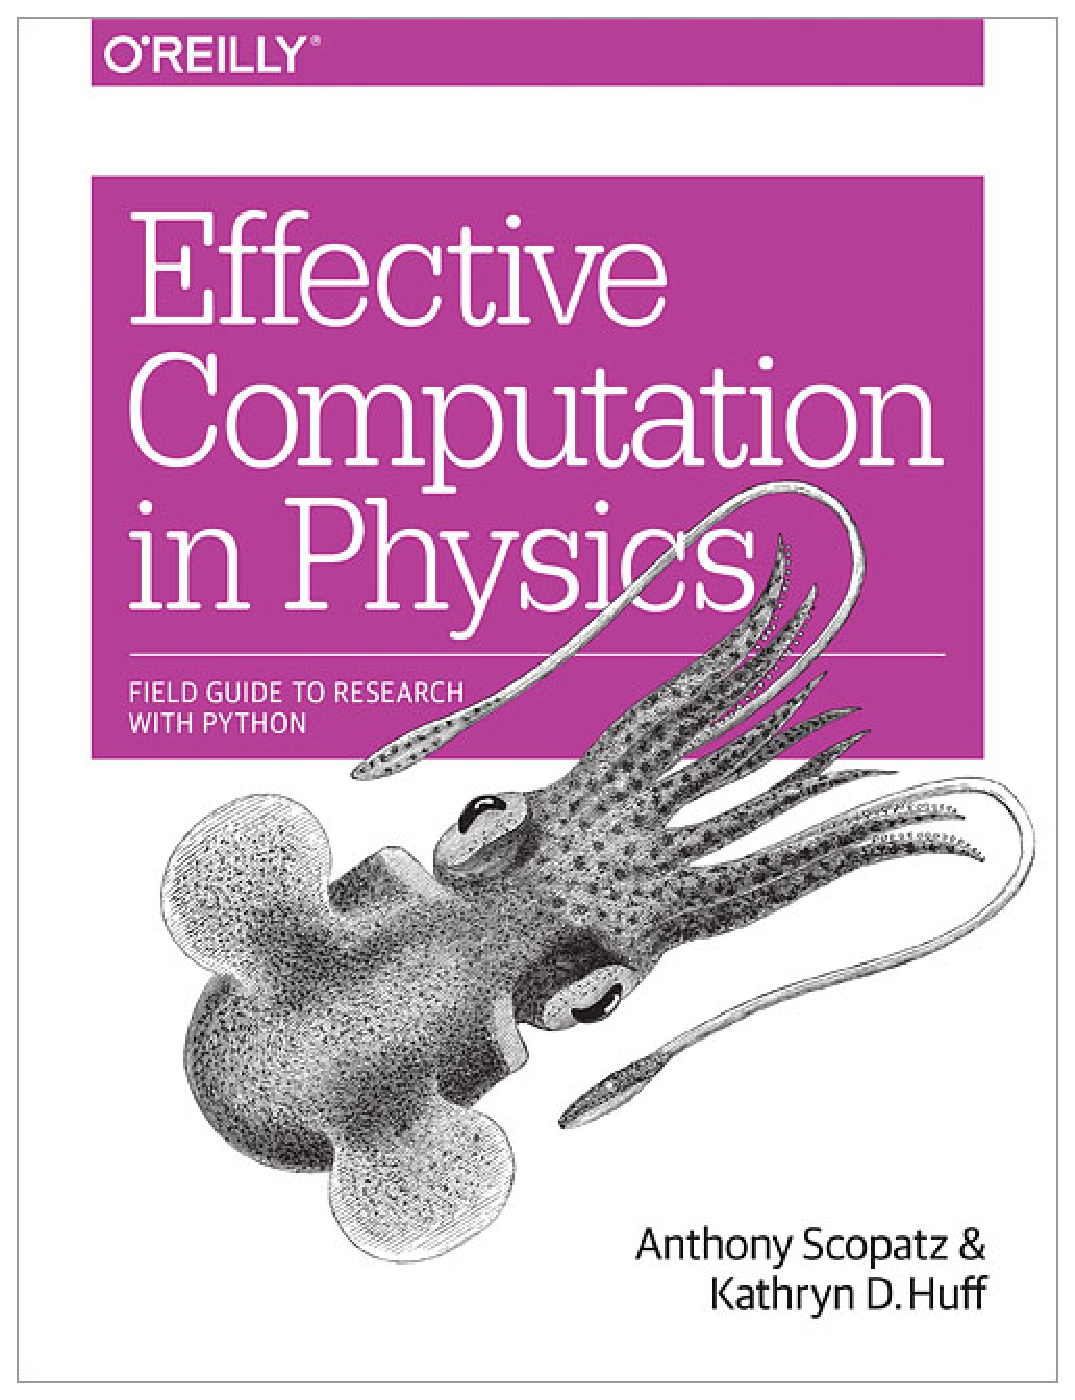
\includegraphics[width=0.4\textwidth]{ecip.eps}
\end{center}
\caption{The textbook for the course is Effective Computation in Physics: A Field Guide To Research in Python}
\label{fig:book}
\end{figure}

The textbook.
\section{Experience}

\subsection{Software Carpentry}

The material and concepts proposed here were heavily influence by the work done
by the Software Carpentry Foundation, an organization that

Software Carpentry has been involed with teaching scientific computing best
practices for over a decade. Students have come from many areas of science and
usually no programming experience is necessary to attend a course. The courses
are typically two days and cover skills for "Doing more with less pain."

Also, the testing, debugging, and collaboration sessions were taught as a part
of a recent workshop at the University of California Berkeley. The students, in
the course of four hours, were able to upload tests and example code to a
version controlled repository and to deploy continuous integration for
automated unit testing.

\section{Conclusions}

This course will equip students with modern concepts that will make them more effective researchers in the data and computing intensive domain of nuclear engineering. These concepts include modules for :

\begin{itemize}
\item getting started with a modern, high-level, object-oriented programming language,
\item getting nuclear engineering work done with sophisticated library design employing powerful data structures,
\item getting correct results by employing workflows that emphasize tests and capture provenance,
\item getting work publication ready with the help of modern computing.
\end{itemize}

By emphasixing projects along the way, the students in this course will learn
to create free and open source tools, verify the functioning of those tools,
and publish them online.  Finally, the syllabus and course textbook are open
and affordable, respectively.

%%%%%%%%%%%%%%%%%%%%%%%%%%%%%%%%%%%%%%%%%%%%%%%%%%%%%%%%%%%%%%%%%%%%%%%%%%%%%%%%
%%%%%%%%%%%%%%%%%%%%%%%%%%%%%%%%%%%%%%%%%%%%%%%%%%%%%%%%%%%%%%%%%%%%%%%%%%%%%%%%
\bibliographystyle{ans}
\bibliography{bibliography} \end{document}
